\documentclass[11pt]{beamer}
\usepackage{tikz}
\usetikzlibrary{fit,positioning}
\usetheme{Singapore}
\usepackage{amssymb,amsmath}
\usepackage{amsthm}
\usepackage{booktabs}
\usepackage{graphicx,float}
\usepackage{epsfig}
\usepackage{pdfpages}
\usepackage{color}
\usepackage{enumerate}
\usepackage{comment}
\usepackage{amstext}
\usepackage{geometry}
\usepackage[lined, ruled]{algorithm2e}
\usepackage{hyperref}
\newcommand{\beq}{\begin{equation}}
\newcommand{\eeq}{\end{equation}}
\newcommand{\beqa}{\begin{eqnarray}}
\newcommand{\eeqa}{\end{eqnarray}}
\newcommand{\bit}{\begin{itemize}\setlength{\itemsep}{0cm}\setlength{\topsep}{0cm}}
\newcommand{\eit}{\end{itemize}}
\newcommand{\benum}{\begin{enumerate}\setlength{\itemsep}{0cm}\setlength{\parsep
}{0cm}}
\newcommand{\eenum}{\end{enumerate}}
\newcommand{\bB}{{\bf B}}
\newcommand{\bv}{{\bf v}}
\newcommand{\bx}{\bf{x}}
\newcommand{\bQ}{{\bf Q}}
\newcommand{\dd}{{\mbox{d}}}
\newcommand{\bK}{{\bf K}}
\newcommand{\bI}{{\bf I}}
\newcommand{\bS}{{\bf S}}
\newcommand{\balpha}{\boldsymbol{\alpha}}
\newcommand{\bR}{{\bf R}}
\newcommand{\bH}{{\bf H}}
\newcommand{\bD}{{\bf D}}
\newcommand{\btheta}{{\boldsymbol{\theta}}}
\newcommand{\btau}{{\boldsymbol{\tau}}}
\newcommand{\bpi}{{\bf \pi}}
\newcommand{\bt}{{\bf t}}
\newcommand\independent{\protect\mathpalette{\protect\independenT}{\perp}}
\def\independenT#1#2{\mathrel{\rlap{$#1#2$}\mkern2mu{#1#2}}}
\newcounter{saveenumi}
\newcommand{\seti}{\setcounter{saveenumi}{\value{enumi}}}
\newcommand{\conti}{\setcounter{enumi}{\value{saveenumi}}}

\resetcounteronoverlays{saveenumi}
\tikzset{onslide/.code args={<#1>#2}{%
  \only<#1>{\pgfkeysalso{#2}} % \pgfkeysalso doesn't change the path
}}

\title{Bayesian analysis of single-molecule experimental data}
\author{\large  S.C. Kou, S. Xie, J. Liu}
\institute{\large Mingwei Tang}
%\institute{ Department of Statistics\\
 % University of Washington\\
  %\texttt{mingwt@uw.edu}}
\date{\today}
\begin{document}
  \maketitle
\begin{frame}
	\frametitle{Overview} % Table of contents slide, comment this block out to remove it
	\tableofcontents % Throughout your presentation, if you choose to use \section{} and \subsection{} commands, these will automatically be printed on this slide as an overview of your presentation
\end{frame}
\section{Background}
\begin{frame}
\frametitle{Molecule: DNA hairpin}
\bit
\item Single-stranded nucleic acid with two ends
\item Two states: closed and open
\item Transitions between two state
\begin{figure}[H]
  \centering
      \includegraphics[width=0.35\textwidth]{twosates}
      \caption{closed(left),open(right)}
\end{figure}

\pause
\item Question: How often does the transition happen? 
\item The state  {\color{red}{can not be observed}}
\eit
 \end{frame}

%\begin{frame}
%\frametitle{Fluroescence lifetime experiments}
%\bit
%\item Using laser impulses to illuminate DNA hairpins
%\item The hairpin will emit photons
%\item Measurement: 
%\bit
%\item Arrival time $t_i$:  Times when a new photon comes
%\item Delay time $\tau_i$: Time between photon being excited and photon being emitted
%\eit
%\item Data $(t_i,\tau_i)^n_{i=0}$ not iid, correlated 
%\eit
%\begin{figure}
%\centering
%\includegraphics[width=0.7\textwidth]{lse}
%\end{figure}
%\end{frame}
{
\setbeamercolor{background canvas}{bg=}
\includepdf[pages=1-17]{flexp.pdf}
}
\begin{frame}
\frametitle{Flurescence lifetime experiments}
\bit
\item The arrival time and delay time depends on the DNA state
\bit
\item Closed state: less arrivals and shorter delay time 
\eit
\item Goal:
\benum
\item Model the state transition
\item Make inference on the parameters related to photon arrival rate and state transition rate 
%\begin{figure}
%\centering
%\includegraphics[width=0.3\textwidth]{twosates}
%\end{figure}
\eenum
\eit
\end{frame}
\section{two-state model}
\subsection{Simple two-state Model}
\begin{frame}
\frametitle{Model 1: Two-state model}
\bit
% \item Use $d_t=1$ and $d_t=2$ to denote closed and open state at time $t$  
% \item The photon arrival time depends on the state of the molecule
\pause
\item 
The transition : continuous-time Markov chain \\
Infinitesimal generator
$$\bQ=\left(\begin{array}{cc}
-k_{12} & k_{12}\\
k_{21}& -k_{21}
\end{array}\right)$$ 
\pause
\item At $t=0$, start from stationary distribution $\bpi=(\pi_1,\pi_2)=(\dfrac{k_{21}}{k_{12}+k_{12}},\dfrac{k_{12}}{k_{12}+k_{12}})$
\item Use $k=k_{12}+k_{21}$ and $\pi_1$ for the transition parameter
\pause
\item State variable $\gamma(t)$: $\gamma(t)=\left\{\begin{array}{ll}
a &   \mbox{Open state at time }t\\
b & \mbox{Closed state at time }t
\end{array}\right.$\\
where $a>b>0$
\eit
\end{frame}

\begin{frame}
\frametitle{Data Oberseved $(\bt,\btau)$}
% $A_0$ denote the parameter of intensity
\bit

\item Photon arrival time $t_i$, $t_0<t_1<\cdots<t_{n}$

\bit
\item Counting process from non-homogeneous Poisson Process
\item Rate $\lambda(t)=A_0/\gamma(t)$ 
\item $A_0>0$: Photon arrival intensity
\eit
\item Delay time $\tau_i$ associated with, $t_i$: $(\tau_0,\ldots,\tau_n)$
\bit
\item $\left[\tau_i|\gamma(t_i)\right]\sim \mbox{Exp}(\gamma(t_i))$
\eit
       \begin{figure}
       	\centering
       	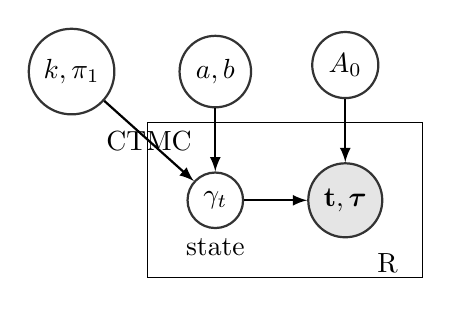
\begin{tikzpicture}
       	\tikzstyle{main}=[circle, minimum size = 5mm, thick, draw =black!80, node distance = 8mm]
       	\tikzstyle{connect}=[-latex, thick]
       	\tikzstyle{box}=[rectangle, draw=black!100]
       	%  \node[main, fill = white!100] (alpha) [label=below:$\alpha$] { };
       	\node[main] (z) [main, fill = white!100,label=below: state] {$\gamma_t$};
              		\node[main, fill = black!10] (w) [right=of z] {$\bt,\btau$ };
       	\node[main] (A0) [above=of w] {$A_0$ };
       	\node[main] (ab) [above=of z] { $a,b$};
       	\node[main] (kpi) [left=of ab] { $k,\pi_1$};
%        \node[main](g1)[left=of z]}{$\gamma$}
       	%  	\node[main](d)
       
       	\path[->]   %(theta) edge [connect] (z)
       	(z) edge [connect] (w)
       	(A0) edge [connect] (w)
       	(ab) edge [connect] (z)
       	(kpi) edge [connect] node {CTMC}  (z);
       	%      \node[rectangle, inner sep=0mm, fit= (z) (w),label=below right:N, xshift=13mm] {};
       	\node[rectangle, inner sep=0.6mm, fit= (z) (w),label=below right:R, xshift=5mm]{};
       	\node[rectangle, inner sep=5mm, draw=black!100, fit =  (z) (w)] {};
       	\end{tikzpicture}
       	\caption{Generative View of the model}
       \end{figure}
\eit
\end{frame}
%\begin{frame}
%\frametitle{Data observed}
%$\gamma(t)$,\mbox{Arrival count}, Delay time vs time
%\begin{figure}
%\centering
%\includegraphics[width=1\textwidth,height=0.5\textwidth]{3p}
%\end{figure}
%\end{frame}
\begin{frame}
\frametitle{Likehood calculation}

\bit
\item Y denote the number of arrivals at time $t$. $\Delta Y_t=Y(t+dt)-Y(t)$ 
\item Likelihood construction $L(\bt,\btau,\gamma|\theta)$
\bit
\item Assumption:\quad $t_{i+1}-t_i \independent \tau_i | \gamma(t_i)$
\item arrival time $t_i$ \qquad $P(\Delta Y_{t_i}=1|\gamma_{t_i})=\frac{A_0}{\gamma(t_i)}dt$
\item delay time $\tau_i$ \qquad  $P(\tau_i|\Delta Y_{t_i}=1,\gamma_{t_i})=\gamma(t_i)\exp(-\gamma(t_i)\tau_i)$
\item no photon arrives in ($t_i$,$t_{i+1}$):  $$P\left(Y^-_{t_{i+1}}-Y_{t_i}=0, \gamma(t_{i+1})|\gamma(t_i)\right)$$
\eit
\begin{figure}
	\centering
	\includegraphics[width=1\textwidth,height=0.3\textwidth]{flexp}
\end{figure}



%\item Likelihood function can be calculated 
%\[
%L(\bt,\btau|\theta)=(\pi_1,\pi_2)\bD_0\bH\left[\prod_{i=0}^{n-1}\exp\{(\bQ-\bH)(t_{i+1}- %t_i)\}\bD_{i+1}\bH\right]\left(\begin{array}{c}
%1\\

%1
%\end{array}\right)\]
%Parameters $\btheta=(a,b,k,A_0)$
\eit
\end{frame}
\begin{frame}
\begin{block}{No arrival probability}
\begin{theorem}
	Let $Y_t$ denotes the total number of arrivals at interval $[0,t)$. Then 
	\begin{align*}
	&P\left(Y^-_{t_{i+1}}-Y_{t_i}=0, \gamma(t_{i+1})|\gamma(t_i)\right)\\
	&=\left[\exp(\bQ-\bH)(t_{i+1}-t_i)\right]_{(\gamma(t_i),\gamma(t_{i+1}))}
	\end{align*}
	where $\bH=\mbox{diag}(A_0/a,A_0/b)$ rate for the arrival time\\
\end{theorem}
\end{block}
\bit
\item Intuition: Kolmogorov forward equation and ODE
\eit
\end{frame}
\begin{frame}
\frametitle{Goal: Inference on parameters}
\bit
\item Parameters $\btheta=(a,b,\pi_1,k,A_0)$
\item Likelihood function 
\begin{align*}
& L(\bt,\btau|\theta)=\sum_{\gamma}L(\bt,\btau,\gamma|\theta)\\
& =(\pi_1,\pi_2)\bD_0\bH\left[\prod_{i=0}^{n-1}\exp\{(\bQ-\bH)(t_{i+1}- t_i)\}\bD_{i+1}\bH\right]\left(\begin{array}{c}
1\\
1
\end{array}\right)
\end{align*}
where 	$\bD_i=\mbox{diag}(a\exp(-a\tau_i),b\exp(-b\tau_i))$ density for the delay time
\eit
\end{frame}


\begin{frame}
\frametitle{Posterior sampling by MCMC}
\bit
\item $\eta(\btheta)$ be the prior distribution 
\item Posterior distribution
$$P(\btheta|\bt,\btau)\propto\eta(\btheta)L(\bt,\btau|\btheta)$$ 
\item Direct sampling is impossible
\item The posterior can be sampled by Metropolis-Hasting algorithm
\eit
\end{frame}

\begin{frame}
\frametitle{Simulations}
\bit
\item 5000 iterations, throw first 2500, draw a sample every 5 iterations
\item the posterior sample covers the true parameter 
\eit
	\begin{figure}
		\centering
		\includegraphics[width=0.70\textwidth]{simple}
	\end{figure}
\end{frame}
%\begin{frame}
%\frametitle{Sampling details}
%\bit
%\item Given the current $\theta=(a,b,\pi,k,A_0)$
%\item Sample $(x,y)$ from two independent gamma distribution with $a,b$ as mean value. Let $a'=\max \{x,y\} $ and $b'=\min\{x,y\}$
%\item Sample $\pi'$, from proposal distribution $\beta(c\pi_1,c(1-\pi_1))$ 
%\eit 
%\end{frame}
\subsection{two-state model with Brownian motion}
\begin{frame}
\frametitle{A question with $A_0$}
\bit
\item Constant photon arrival intensity? 
\item The DNA molecule will move in the focal volume
\item The arrival intensity varies with molecule location
\begin{figure}
\centering
\includegraphics[width=0.4\textwidth]{br3d}
\end{figure}  
 \item Use $A(t)=A_0\alpha(t)$ $\quad \alpha(t)\in (0,1]$


\eit
\end{frame}
\begin{frame}
 
\bit
\item $(B_x(t),B_y(t),B_z(t))$ position at time $t$.  $$\alpha(t)=\exp\left\{-\dfrac{B^2_x(t)+B^2_y(t)}{2w^2_{xy}}-\dfrac{B^2_z(t)}{2w_z^2}\right\}$$
%\item $w_{xy}$ and $w_z$  : the radius and height of focal volume
\item Motion of the Molecule: {\color{red} Brownian motion}
\bit
\item Use a three independent Brownian motion $(B_x(t),B_y(t),B_z(t))$ to model the location
\item $dB_x(t)=\sigma dW_t$
%\item Variance constant $\sigma$: related to velocity of the molecule (known)
\eit
\item $w_{xy},w_z$ are known
\eit
\end{frame}
\begin{frame}
	\bit
	\item Arrival time $t_i$ \qquad $P(\Delta Y_{t_i}=1|\gamma_{t_i},\alpha_{t_i})=A(t_i)/\gamma(t_i)$
	\eit
       \begin{figure}
       	\centering
       	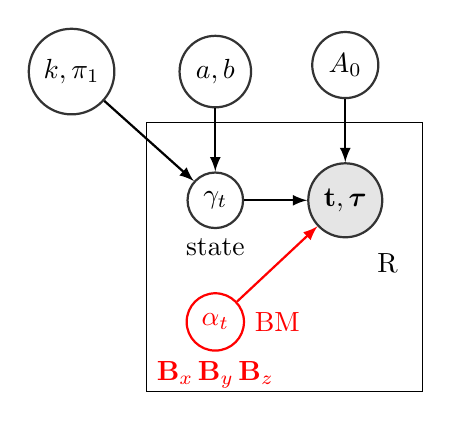
\begin{tikzpicture}[highlight/.style={draw=red, text=red}]
       	\tikzstyle{main}=[circle, minimum size = 5mm, thick, draw =black!80, node distance = 8mm]
       	\tikzstyle{connect}=[-latex, thick]
       	\tikzstyle{box}=[rectangle, draw=black!100]
       	%  \node[main, fill = white!100] (alpha) [label=below:$\alpha$] { };
       	\node[main] (z) [main, fill = white!100,label=below: state] {$\gamma_t$};
       	\node[main, fill = black!10] (w) [right=of z] {$\bt,\btau$ };
       	\node[main] (A0) [above=of w] {$A_0$ };
       	\node[main] (ab) [above=of z] { $a,b$};
       	\node[main] (kpi) [left=of ab] { $k,\pi_1$};
     %  	\node[main](xt)[left=of z,label=below: EB]{$x_t$};
      % 	\node[main](lx)[left=of kpi,label=below: OU para]{$\lambda,\xi$};
       	\node[main](al)[highlight,below=of z,label=below:$\color{red}\bB_x\,\bB_y\,\bB_z$,label=right:\color{red}BM]{\color{red}$\alpha_t$};
       	%        \node[main](g1)[left=of z]}{$\gamma$}
       	%  	\node[main](d)
       	
       	\path[->]   %(theta) edge [connect] (z)
       	(z) edge [connect] (w)
       	(A0) edge [connect] (w)
       	(ab) edge [connect] (z)
       	(kpi) edge [connect] (z)
       	(al) edge[connect,highlight] (w);
       	%      \node[rectangle, inner sep=0mm, fit= (z) (w),label=below right:N, xshift=13mm] {};
       	\node[rectangle, inner sep=0.6mm, fit= (z) (w),label=below right:R, xshift=5mm]{};
       	\node[rectangle, inner sep=5mm, draw=black!100, fit =(al)  (z) (w)] {};
       	\end{tikzpicture}
       	\caption{Generative view of the two-state Model with Brownian motion}
       \end{figure}
\end{frame}

\begin{frame}
\frametitle{Likelihood contruction}
\bit
\item Approximation: $\alpha(t)=\alpha(t_i)$ for $t\in(t_i,t_{i+1})$ 
\item Conditioning on $\alpha(t)$: substitute $A_0$ with $A(t_i)=A_0\alpha(t_i)$
\pause
\begin{align*}
& L(\bt,\btau|\theta,\alpha(t))\\
&=(\pi_1,\pi_2)\bD_0{\color{red}\bH_0}\left[\prod_{i=0}^{n-1}\exp\{(\bQ-{\color{red}\bH_i})(t_{i+1}- t_i)\}\bD_{i+1}{\color{red}\bH_{i+1}}\right]\left(\begin{array}{c}
1\\
1
\end{array}\right)
\end{align*}
where $H_i=\left(\begin{array}{cc}
A(t_i)/a & 0\\
0 & A(t_i)/b
\end{array}\right)$
\eit
\end{frame}
\begin{frame}
\bit
\pause
\item Posterior distribution has the form
\begin{align*}
P(\theta|\bt,\btau)\propto & \int \eta(\theta)L(\bt,\tau|\theta,\alpha(t))P(\alpha(t))d(\alpha(t))\\
&= \int \eta(\theta)L(\bt,\tau|\theta,\alpha(t))P(\bB(t))d(\bB(t))
\end{align*}
\pause
\item Method: Data augmentation
\bit
\item Draw $\theta$ conditioning on current diffusion $(B_x,B_y,B_z)$
$$\btheta\sim[\btheta|\bB,\bt,\btau]\propto \eta(\btheta)L(\bt,\btau|\btheta,\alpha_t)$$
\item Draw the diffusion $(B_x,B_y,B_z)$ conditioning on the current value of $\btheta$,
$$[B_x,B_y,B_z|\btheta,\bt,\btau]\sim L(\bt,\btau|\btheta,\alpha(t))
P(B_x)P(B_y)P(B_z)$$
\eit
\eit
\end{frame}

\section{Continuous diffusive model}
\begin{frame}
\frametitle{Model2: Continuous diffusive model}
State transition: non-homogeneous CTMC
\bit 
\item Intuition: Transition depends on energy barrier $x_t$
\begin{figure}
\centering
\includegraphics[width=0.5\textwidth]{eb}
\end{figure}
\item The energy barrier changes with time
\eit
\end{frame}

\begin{frame}
\frametitle{Model the change of Energy barrier}
\bit
\item $x_t$ modeled by Ornstein-Uhlenbeck process $\lambda>0,\xi>0$
$$\mbox{d}x_t=-\lambda x_t\dd t+\sqrt{2\lambda\xi}\dd W_t$$
\pause
\item Continuous diffusive model:

 The transition rate is no longer constant 
 $$\bQ(t)=\left(\begin{array}{cc}
 -k_{12}{\color{red}\exp(-x(t))} &k_{12}{\color{red}\exp(-x(t))} \\
 k_{21}{\color{red}\exp(-x(t))}  & -k_{21}{\color{red}\exp(-x(t))} 
 \end{array}\right)$$

\item At $t=0$, the OU-process starts at stationary distribution \[x_0\sim N(0,\xi)\]

\eit

\end{frame}


\begin{frame}
\frametitle{A generative view of the model}
 Continuous diffusion model
    \begin{figure}
    \centering
  	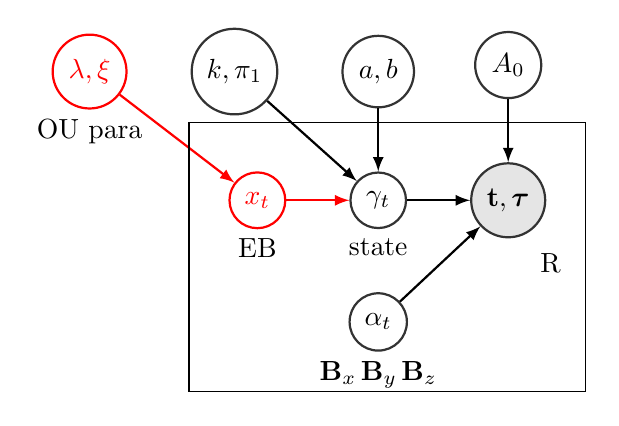
\begin{tikzpicture}[highlight/.style={draw=red, text=red}]
  	\tikzstyle{main}=[circle, minimum size = 5mm, thick, draw =black!80, node distance = 8mm]
  	\tikzstyle{connect}=[-latex, thick]
  	\tikzstyle{box}=[rectangle, draw=black!100]
  	%  \node[main, fill = white!100] (alpha) [label=below:$\alpha$] { };
  	\node[main] (z) [main, fill = white!100,label=below: state] {$\gamma_t$};
  	\node[main, fill = black!10] (w) [right=of z] {$\bt,\btau$ };
  	\node[main] (A0) [above=of w] {$A_0$ };
  	\node[main] (ab) [above=of z] { $a,b$};
  	\node[main] (kpi) [left=of ab] { $k,\pi_1$};
  	\node[main](xt)[highlight,left=of z,label=below: EB]{$x_t$};
  	\node[main](lx)[highlight,left=of kpi,label=below: OU para]{$\lambda,\xi$};
  	\node[main](al)[below=of z,label=below:$\bB_x\,\bB_y\,\bB_z$]{$\alpha_t$};
  	%        \node[main](g1)[left=of z]}{$\gamma$}
  	%  	\node[main](d)
  	
  	\path   %(theta) edge [connect] (z)
  	(z) edge [connect] (w)
  	(A0) edge [connect] (w)
  	(ab) edge [connect] (z)
  	(kpi) edge [connect] (z)
  	(lx) edge [connect,highlight] (xt)
  	(xt) edge [connect,highlight] (z)
  	(al) edge[connect] (w);
  	%      \node[rectangle, inner sep=0mm, fit= (z) (w),label=below right:N, xshift=13mm] {};
  	\node[rectangle, inner sep=0.6mm, fit= (z) (w),label=below right:R, xshift=5mm]{};
  	\node[rectangle, inner sep=5mm, draw=black!100, fit =(al) (xt) (z) (w)] {};
  	\end{tikzpicture}
  	\caption{Generative View of the model}
  \end{figure}
\end{frame}

\begin{frame}
\frametitle{Posterior for continuous diffusive model}
\bit
\item Likelihood construction: Approximation $\bQ(t)=\bQ(t_i), t\in (t_i,t_{i+1})$
\begin{align*}
& L(\bt,\btau|\theta,\alpha(t),\bx_t)\\
&=(\pi_1,\pi_2)\bD_0\bH_0\left[\prod_{i=0}^{n-1}\exp\{({\color{red}\bQ(t_i)}-\bH_i)(t_{i+1}- t_i)\}\bD_{i+1}{\bH_{i+1}}\right]\left(\begin{array}{c}
1\\
1
\end{array}\right)
\end{align*}
\pause
\item Posterior distribution
\begin{align*}
& P(\btheta,\lambda,\xi|\bt,\btau)\propto\\ 
&\int\int \eta'(\btheta,\lambda,\xi)L(\bt,\btau|\theta,\alpha_t,\bx_t)P(\alpha_t)P(\bx_t|\lambda,\xi)d(\alpha_t)d(\bx_t)
\end{align*}
\item Method: Data augmentation 
\eit
\end{frame}

\begin{frame}
\frametitle{Sampling Steps}

\benum
\item Sample parameter $\btheta$
$$\btheta\sim[\btheta|\lambda,\xi,\bB,x_t,\bt,\btau]\propto \eta'(\btheta,\lambda,\xi)L(\bt,\btau|\theta,\alpha_t,x_t)$$

\item Sample diffusion parameter $\lambda,\xi$
$$(\lambda,\xi)\sim[\lambda,\xi|\btheta,\bB,x_t,\bt,\btau]\propto \eta'(\btheta,\lambda,\xi)P(x_t|\lambda,\xi)$$

\item Sample the the Brownian motion path
$$\bB\sim [\bB|\btheta,\lambda,\xi,x_t,\bt,\btau]\propto L(\bt,\btau|\theta,\alpha_t,x_t) P(\bB)$$

\item Sample the energy barrier path
$$x(t)\sim[x_t|\btheta,\lambda,\xi,\bB,\bt,\btau]\propto L(\bt,\btau|\theta,\alpha_t,x_t)P(x_t|\lambda,\xi)$$

\eenum
\end{frame}


\section{Experiment}
\begin{frame}
	\frametitle{Association with two states model}
	$$dx_t=-\lambda x_tdt+\sqrt{2\lambda\xi}dW_t$$
	If $\xi \simeq 0$
	\bit
	\item The stationary distribution $N(0,\xi)$ will degenerate to 0
	\item The SDE has solution $x_t=0$
\pause
	\item The infinitesimal $Q(t)$
	\[
	\bQ(t)=\left(\begin{array}{cc}
	-k_{12} & k_{12}\\
	k_{21}& -k_{21}
	\end{array}\right)
	\]
	\pause
	\item Exactly the two-state model! 
	\eit
\end{frame}
\begin{frame}
	\frametitle{Model Comparision}
	\benum
	\pause
	\item By checking the value of $\xi$
	
	$\bH_0: \xi=0$ two-state model\\
	$\bH_1:\xi>0$ continuous diffusion model 
	\pause
	\item By comparing Bayes factor 	$$\mbox{BF}=\dfrac{P(\bt,\btau|M_1)}{P(\bt,\btau|M_2)}$$
	
	where $M_1$ is the two state model, $M_2$ is the continuous diffusive model
	\eenum
\end{frame}
\subsection{Simulated data}
\begin{frame}
\frametitle{Details on priors and other parameters}
\benum
\item Prior issues
\benum
\item Informative prior for $\btheta=(a,b,\pi_1,k,A_0)$
\bit
\item $a\sim \Gamma(2,1)$
\item $b\sim \Gamma(1.5625,1.5625)$
\item $\pi_1\sim \mbox{beta}(0.89,0.89)$
\item $\pi_1\sim \mbox{Exp}(1/40000)$
\item $A_0\sim \Gamma(1.96,5.6\times10^{-5})$
\eit
\item Less information for $\lambda$,$\xi$. 
\bit
\item $\lambda\sim \Gamma(40,0.5)$
\item $\xi\sim \Gamma(2,1)$
\eit
\eenum
\item Other parameters
\bit
\item Brownian motion parameters: $w_{xy}=310,w_z=1760$
\item BM constant $\sigma^2$ is not given, set as 1000
%\item Initial condition for the Brownian motion: not known
\eit
\eenum
\end{frame}

\begin{frame}
\frametitle{Experiment 1: Simulated datasets}
\bit
\item Simulate {\color{red}50} sequences of $(\bt,\btau)$s 
\item Each sequence is simulated from {\color{red} two-state BM model} with $t_{max}<0.05$
\item The number of observations in each datasets varies from $1000\sim 5000$
% \item The conditional likelihood function is the product of the likelihood on each sequence $(\bt,\btau)$
\item Run both two-state model and continuous diffusion model for 5000 iterations
\eit
\end{frame}


\begin{frame}
\frametitle{two-state BM model}
\bit
\item Posterior samples for $(a,b,\pi_1,k,A_0)$
	\begin{figure}
		\centering
		\includegraphics[width=0.8\textwidth,height=0.5\textwidth]{m4simu1}
	\end{figure}
%\begin{figure}
%	\centering
%	\begin{minipage}{0.45\textwidth}
%		\includegraphics[width=1.05\textwidth]{m4simu1}
%	\end{minipage}
%	\begin{minipage}{0.45\textwidth}
	%	\includegraphics[width=1.05\textwidth]{m4simu2}
	%		\end{minipage}
%\end{figure}
\eit
\end{frame}


\begin{frame}
	\frametitle{Continuous diffusive model}
	\bit
	\item Posterior samples for $(a,b,\pi_1,k,A_0,{ \color{red}\xi})$
	\begin{figure}
		\centering
		\includegraphics[width=0.8\textwidth,height=0.5\textwidth]{m4simu2}
	\end{figure}
$\mbox{BF} = 0.99$, no significant difference between the two model
\eit
\end{frame}
\subsection{Real data}
\begin{frame}
\frametitle{Experiment 2: Real data}
\bit
\item 50 real datasets from Xie's lab at Harvard University 
\item Each contains a sequence of 1815 pairs of $(t_i,\tau_i)$
\item Run both two-state model and continuous diffusion model for 5000 iterations
\eit
\end{frame}

\begin{frame}
	\frametitle{two-state BM model}
	\bit
	\item posterior samples $(a,b,\pi_1,k,A_0)$
		\begin{figure}
			\centering
			\includegraphics[width=0.8\textwidth,height=0.5\textwidth]{real1}
		\end{figure}
%	\begin{figure}
%		\centering
%		\begin{minipage}{0.45\textwidth}
%			\includegraphics[width=1.05\textwidth]{real1}
%		\end{minipage}
%		\begin{minipage}{0.45\textwidth}
%			\includegraphics[width=1.05\textwidth]{real2}
%		\end{minipage}
%	\end{figure}
	\eit
\end{frame}
%\begin{frame}
%	\frametitle{Real data, two-state model}
%	\begin{figure}
%				\centering
%					\includegraphics[width=0.8\textwidth]{real1}
%	\end{figure}
					
%\end{frame}
\begin{frame}
	\frametitle{Continuous diffusive model}
	\bit
\item Posterior samples for $(a,b,\pi_1,k,A_0,{\color{red} \xi})$
	\begin{figure}
		\centering
		\includegraphics[width=0.8\textwidth]{real2}
	\end{figure}
	\eit
\end{frame}

\begin{frame}
\bit
\item Comparing posterior mean

{\small
%\begin{table}
%		\begin{tabular}{@{}llllll@{}}
%			\toprule
%			& $a$ & b & $\pi_1$ & k & $A_0$ \\ \midrule
%			prior & $\Gamma(1,0.5)$ &$\Gamma(1.56,1.56)$   &  $\mbox{Beta}(0.89,0.89)$   & $\mbox{Exp}(1/4000)$  &  $\Gamma(1.96,\frac{7}{12500}$     \\
%			twostateBM   & 1.367   & 0.289  & 0.604    & 26744   & 37421      \\
%			Con-diff    & 1.405  & 0.289  & 0.605       &  25830  & 37235      \\ \bottomrule
%		\end{tabular}
%	\end{table}}
	\begin{table}
	\begin{tabular}{cccc}
	\toprule
			para& prior & twostateBM &	Con-diff  \\ \midrule
			a& $\Gamma(1,0.5)$ & 1.367 & 1.405 \\
			b& $\Gamma(1.56,1.56)$ & 0.289 &  0.289 \\
			$\pi_1$ &  $\mbox{Beta}(0.89,0.89)$ & 0.604 & 0.605   \\	
			k& $\mbox{Exp}(1/4000)$ & 26744  &25830 \\
			$A_0$ & $\Gamma(1.96,\frac{7}{12500})$ & 37421 & 37235 \\ 
			\bottomrule
			\end{tabular}
	\end{table}
	}
	\item $\mbox{BF} = 0.023$, evidence for continuous diffusive model
	\eit
\end{frame}
\begin{frame}
	\frametitle{Summary}
	\bit
	\item Fluorescence experiment
	\item Two models: (Likelihood function)
	\bit
	\item two-state model: CTMC transition\\
	Two state model with BM
	\item Continuous diffusion model: OU-process for energy barrier
	\eit
	\item Sampling from posterior distribution
	\bit
	\item Metropolis-hasting algorithm
	\item Data Augmentation algorithm
	\eit
	\item Model selection: 
	\bit 
	\item By $\xi$
	\item Bayes factor
	\eit
	\item Experiment : continuous diffusive model fits better on the real data
	\eit
\end{frame}
\section{Discussion}
\begin{frame}
\frametitle{Discussion}
\benum
\item Pros
\bit 
\item First Bayesian model to study s single-molecule experiment
\item Can incorporate many conditions in the experiment (BM, OU for EB)
\item Can be extended to model other counting process with latent structure
\item The computation cost for each iteration is $\mathcal{O}(n)$
\eit
\item Cons
\bit
\item Low efficiency in component-wise update in the Brownian motion path 
\item Sensitive to prior $(\lambda,\xi)$ 
\item Some other models between two-states model and continuous diffusive model 
\eit
\eenum
\end{frame}
\begin{frame}
\begin{center}
{\Huge Thank you!}
\end{center}

\end{frame}
\section{Questions and answers}
\begin{frame}
	\frametitle{Componentwise update}
	For $i=0,1,\ldots,n$
	\benum
	\pause
	\item Propose a new location $B_i'=(B'_x,B_y',B_z')$ for the $i$th time point $B(t_i)=(B_x(t_i),B_y(t_i),B_z(t_i))$\\
	Calculate $\alpha'$ at time $t_i$
	\pause
	\item Calculate M-H ratio
	$$r=\dfrac{L(\bt,\btau|\theta,\alpha'_t)P(B'_x)P(B'_y)P(B'_z)T(B'\rightarrow B(t_i))}{L(\bt,\btau|\theta,\alpha_t)P(B_x)P(B_y)P(B_z)T(B\rightarrow B'(t_i))}$$
	\item Sample $U\sim U(0,1)$. \\
	Update $B(t_i)$ to $B'$ when $U<r$
	\eenum
\end{frame}

\begin{frame}
	\frametitle{The diffusion Path}
	\bit
	\item Identifiability issues
	\bit
	\item The path of $\alpha(t)$ can be is related conditional likelihood. We can find a path will high posterior probability, if $(B_x(t_0),B_y(t_0),B_z(t_0))$ is fixed. 
	\item Notice $\alpha(t)=\exp\left\{-\frac{B^2_x(t)+B^2_y(t)}{2w^2_{xy}}-\frac{B^2_z(t)}{2w_z^2}\right\}$. 
	\item The underlying Brownian path is not identifiable. Multiple paths for the sample $\balpha_t$
	\eit
	\eit
\end{frame}
\begin{frame}
\frametitle{The diffusion path}
Problems related to component-wise update
\bit
\item Low acceptance rate  
	\bit
	\item $r=\dfrac{L(\bt,\btau|\theta,\alpha'_t)}{L(\bt,\btau|\theta,\alpha_t)}\cdot\dfrac{P(B'_x)P(B'_y)P(B'_z)}{P(B_x)P(B_y)P(B_z)}$ if using symmetric proposed density function
	\item 	$P(\bB_x)=(2\pi)^{n/2}\exp\left[-\dfrac{1}{2\sigma^2}\sum_{i=0}^{n-1}\dfrac {[B_x(t_{i+1})-B_x(t_i)]^2}{\Delta t_i}\right]$
	\item $L(\bt,\btau|\theta,\alpha_t)$not sensitive to $\alpha$, $P(B_x),P(B_y),P(B_z)$ sensitive to the change of $B_x,B_y,B_z$
	\item Easily stuck in a "smooth" Brownian motion path
	\eit
	\eit
%\begin{figure}

%\end{figure}

\end{frame}

\begin{frame}
\frametitle{two-stage update}
\benum
\item stage one:\\ 
Propose a change $B'_x\sim N\left(B_x(t_{i-1}),\sigma^2(t_i-t_{i-1})\right)$\\
$u\sim U(0,1)$. Accept the change is $u\leq \dfrac{L(\bt,\btau|\theta,\alpha'_t)}{L(\bt,\btau|\theta,\alpha_t)}$
\item stage two: M-H method with component-wise update

\begin{figure}
\centering
\includegraphics[width=0.8\textwidth]{brpath}
\end{figure}
\eenum
\end{frame}

\begin{frame}
\frametitle{Why bayesian method?}
\bit
\pause
\item Tradition methods: 
\bit
\item Method of Moments
\item Maximum likelihood estimation directly
\item EM
\eit
\pause
\item Why Bayesian?
\bit 
\item Closed from likelihood function
\item The model can be written as a generative model
\item \color{red}{Informative prior}
\eit
\eit
\end{frame}
\begin{frame}
\frametitle{Computation cost}
%\bit 
%\item Likelihood
%\begin{align*}
%& L(\bt,\btau|\theta,\alpha(t))\\
%&=(\pi_1,\pi_2)\bD_0{\color{red}\bH_0}\left[\prod_{i=0}^{n-1}\exp\{(\bQ-{\color{red} \bH_i})(t_{i+1}- t_i)\}\bD_{i+1}{\color{red}\bH_{i+1}}\right]\left(\begin{array}{c}
%1\\
%1
%\end{array}\right)
%\end{align*}
%\item Computation cost for each model
%\eit
{\small
\begin{table}
\centering
%\caption{My caption}
%\label{my-label} %
%\begin{tabular}{lll l}
%\hline
%model & $\#$ of paras & $\#$updates/iter & computing/iter \\ \hline
%simple two-state & 5 & 5 & $\mathcal{O}(n)$   \\
%two-state BM & 5 & 5+3(n+1) & $\mathcal{O}(n)$   \\
%cont-diffusive& 7 & 7+4(n+1) & $\mathcal{O}(n)$  
% \end{tabular}
\begin{tabular}{llll}
\hline
 & simple twostate & twostateBM & cont-diff\\ \hline
$\#$ofparas & 5 & 5 & 7\\
$\#$ofupdates/iter & 5 & 3n+6 & 4n+11\\
cpu-cost(naive)& $\mathcal{O}(n)$&$\mathcal{O}(n^2)$ & $\mathcal{O}(n^2)$\\
cpu-cost(opt)&$\mathcal{O}(n)$&$\mathcal{O}(n)$&$\mathcal{O}(n)$\\ \hline

\end{tabular}
\end{table} }
\end{frame}

\begin{frame}
\frametitle{Backward-forward algorithm}
\bit
\item Likelihood function  $(\pi_1,\pi_2)\left[\prod_{i=0}^{n-1}\bD_i{\color{red}\bH_i}\exp\{(\bQ-{\color{red}\bH_i})(t_{i+1}- t_i)\}\right]\bD_{n}{\color{red}\bH_{n}}\left(\begin{array}{c}
1\\
1
\end{array}\right)$	
\item 	Compute {\it backwards} a sequence of matrices $K_i$ by recursion
		\begin{align*}
		\left\{
	\begin{array}{ll}
			\bK_{n+1}=\bI, \\ 
			\bK_n=\bD_n\bH_n,\\
			\bK_i=\bD_i\bH_i\exp\{(\bQ-\bH_i)\Delta t_i\}\bK_{i+1}, & i=n-1,\ldots,1,0
		\end{array}
		\right.		
	\end{align*}
\eit
\end{frame}

\begin{frame}
\bit
\item Forward calculation
\benum
\item Propose a change $\bB'=(B_x',B_y',B_z')$ for the $i$th time point $(B_x(t_i),B_y(t_i),B_z(t_i))$, calculate $\alpha'_{t_i}$,$\bH'$ based on $(B_x',B_y',B_z')$.
\item Compute 
			$$\bR=\left\{\begin{array}{ll}
				\bD_i\bH_i\exp\{(\bQ-\bH_i)\Delta t_i\}& \mbox{if } i<n, \\
				\bD_n\bH_n & \mbox{if } i=n,
			\end{array}
			\right.$$
			$$\bS=\left\{\begin{array}{ll}
				\bD_i\bH'_i\exp\{(\bQ-\bH'_i)\Delta t_i\}& \mbox{if } i<n, \\
				\bD_n\bH'_n & \mbox{if } i=n,
			\end{array}
		\right.$$
	and\\
				$L(\bt,\btau|\btheta,\balpha'_t)=\bv_i\bS \bK_{i+1}\left(\begin{array}{c}
						1\\
						1
						\end{array}\right)$ and $L(\bt,\btau|\btheta,\balpha_t)=\bv_i\bR  \bK_{i+1}\left(\begin{array}{c}
						1\\
						1
						\end{array}\right)$.		
\eenum
\eit
\end{frame}

\begin{frame}
\bit
	\item Compute MH ratio
						\begin{align*}\label{MH2}
						r=\dfrac{L(\bt,\btau|\btheta,\balpha'_t)P(\bB'_x)P(\bB'_y)P(\bB'_z)T(\bB_i'\rightarrow \bB(t_i))}{L(\bt,\btau|\btheta,\balpha_t)P(\bB_x)P(\bB_y)P(\bB_z)T(\bB_i\rightarrow \bB'(t_i))},
						\end{align*}
						where $T(\cdot\rightarrow\cdot)$ is the transition density of the proposal distribution. 
						\item Generate $u\sim \mbox{Uniform}(0,1)$. \\
						If $u<\min(1,r)$, then update $\bB(t_i)$ to $\bB'$ and $\bv_{i+1}=\bv_i\bS$.\\
						Otherwise, keep $\bB(t_i)$ unchanged and $\bv_{i+1}=\bv_i\bR$
\eit
\end{frame}
\begin{frame}
\frametitle{Sensitivity issues}
Likelihood function: 
\bit
\item Sensitive to $a,b$ since $\btau$ mainly contains information for $a,b$
\item Not sensitive to $\pi,k,A_0$
\item Not sensitive to the $\alpha(t)$ path and OU path $x_t$
\eit
\end{frame}
\begin{frame}
\frametitle{Why combining multiple datasets}
\benum
\item Observed sequence $(t_i,\tau_i)$ not i.i.d
\item Brownian motion model, as $t\rightarrow \infty$, $\alpha(t)\rightarrow 0$ with high probability
\item Identifiability issues for the energy barrier path 
\eenum
\end{frame}
%\begin{frame}
%	\frametitle{}
	
%\end{frame}
\end{document}